\documentclass[11pt,twocolumn,letterpaper]{article}

\usepackage{cvpr}
\usepackage{times}
\usepackage{epsfig}
\usepackage{graphicx}
\usepackage{amsmath}
\usepackage{amssymb}
\usepackage{mathtools}
\usepackage{array}
\usepackage{multirow}
\usepackage{float}

% Box for the confusion matrix
\newcommand\MyBox[2]{
	\fbox{\lower0.75cm
		\vbox to 1.7cm{\vfil
			\hbox to 1.7cm{\hfil\parbox{1.1cm}{#1#2}\hfil}
			\vfil}%
	}%
}

\usepackage{etoolbox}
\makeatletter
\patchcmd{\@verbatim}
{\verbatim@font}
{\verbatim@font\scriptsize}
{}{}
\makeatother

% Include other packages here, before hyperref.

% If you comment hyperref and then uncomment it, you should delete
% egpaper.aux before re-running latex.  (Or just hit 'q' on the first latex
% run, let it finish, and you should be clear).
\usepackage[breaklinks=true,bookmarks=false]{hyperref}

\cvprfinalcopy % *** Uncomment this line for the final submission

\def\cvprPaperID{****} % *** Enter the CVPR Paper ID here
\def\httilde{\mbox{\tt\raisebox{-.5ex}{\symbol{126}}}}


% Pages are numbered in submission mode, and unnumbered in camera-ready
%\ifcvprfinal\pagestyle{empty}\fi
\setcounter{page}{1}
\begin{document}

%%%%%%%%% TITLE
\title{Assignment 2 \\ COMP SCI 7209 - Introduction to Statistical Machine Learning\\ AdaBoost implementation}

\author{Julian Cabezas Pena\\
Student ID: a1785086\\
University of Adelaide, SA 5005 Australia\\
{\tt\small julian.cabezaspena@student.adelaide.edu.au}
% For a paper whose authors are all at the same institution,
% omit the following lines up until the closing ``}''.
% Additional authors and addresses can be added with ``\and'',
% just like the second author.
% To save space, use either the email address or home page, not both
}

\maketitle
%\thispagestyle{empty}


%%%%%%%%% BODY TEXT
\section{Understanding of the AdaBoost method}

One of the most common applications of machine learning techniques is their utilization in classification problems, where an algorithm takes a vector or array of input data, and assigns it to one or many discrete classes \cite{Bishop2006}. These algorithms usually depend on the availability of labelled data ans its corresponding attributes or explanatory variables, and thus are considered as supervised learning \cite{Hastie2009}. 

Boosting is based on the simple premise of combining the output of several weak classifiers, such as simple decision trees, to generate a most accurate "committee" . In these kind of algorithm, a set of weak learners are trained in sequence to decrease the error with each iteration or now weak learner \cite{Hastie2009}. One of the most common boosting algorithms is the Adaptative Boosting (AdaBoost), that iteratively calls a base or weak algorithm, that is fitted on the dataset. In each of the iterations the algorithm is trained over a different set of weights on a defined distribution, that is adjusted to assign a larger weight to the misclassified samples in the previous iteration \cite{Freund1999}.

The AdaBoost algorithm can be considered a a "voting algorithm", that in its time outperformed other state-of-the-art algorithms, such as the Support vector Machine (SVM) for classification tasks \cite{Schapire1998}, as the misclassified samples, that are close to the margin, receive a larger weights, thus increasing their chance of being correctly classified in the next iteration. Moreover, Schapire et al \cite{Schapire1998} explain that the AdaBoost "Boosts the margin" increasing the distance between classes in each iteration. The same authors explain that this algorithm usually reach 100\% train accuracy even with few iterations, while reducing the test error with further iterations. On the other hand, authors such as Mason \textit{et al} \cite{Mason2000} consider the AdaBoost algorithm to perform gradient descent, with each learner added to the ensemble being considered as a step in the optimization process.

%-------------------------------------------------------------------------


\section{Algorithmic Description of the AdaBoost method}

In this paper, the implementation of the AdaBoost algorithm follows the steps described by Freund and Schapire \cite{Freund1999}. If we have a matrix of features $X$ containing $n$ observations and a label $y$ also containing $n$ observations, and we have that $y = \{-1,+1\}$. We can train $M$ weak or base learners ($G(x)$).

Firstly, the weights are initialized as $W_1 = 1/n$. 

Then for each iteration of the algorithm $m = 1,2,3...M$:

- Train a weak learner $G_m(x)$ using the weights $W_m$

- Calculate the error using:

\begin{equation}
	err_m = \sum_{i=1}^{N} W_i I(y_i \neq G_m(x_i))
\end{equation}

- Calculate the $\alpha$ value as

\begin{equation}
	\alpha_m = \frac{1}{2}ln(\frac{1-err_m}{err_m})
\end{equation}

- Update the weights of the samples using the following equation, that results in the weights adding a total of 1:

\begin{equation}
	W_{m+1} (i) = \frac{W_m exp(-\alpha_m y_i g_m(x_i))}{\sum_{i=1}^{N} W_i}
\end{equation}

Then, to generate the prediction using the ensemble of weak learners, the $\alpha$ of each iteration acts like the weights of each learner, as:

\begin{equation}
	G(X) = sign(\sum_{m=1}^{M} \alpha_m g_m(x))
\end{equation}

Thus, the output of the AdaBoost algorithm can be -1 or +1

\subsection{Weak learner: Decision Stump}

In order to train the AdaBoost algorithm, a base learner, that is usually slightly better than random guessing, has to be applied \cite{Freund1999}. In this case, a simple decision stump was implemented. The decision stump is a supervised learning algorithm that involves using a single feature to classify the data, using a threshold that minimizes the error or the amount of misclassifications in the data \cite{Oliver1994}, they can be also interpreted as decision trees of depth equal to one. This kind of weak learner is commonly used in implementations of AdaBoost \cite{Hastie2009}

In this case, to construct the decision tree, a greedy approach was used. The decision stump algorithm goes feature by feature testing a number of threshold values equivalent to the number of samples, starting from the minimum value and finishing in the maximum value, the threshold values that are tested are evenly distributed between these values. Additionally, the threshold values are tested using two different directions or polarities (classifying the samples to -1 or +1 depending on the side of the threshold they are located)

The error of the classification, used to pick the best threshold, direction and feature, was measured using the following equation \cite{Freund1999}

\begin{equation}
	err = \sum_{i=1}^{N} W_i I(y_i \neq g(x_i))
\end{equation}

Where $g()$ is the weak learner and $W$ the set of weights in the corresponding iterations

\section{AdaBoost implementation and analysis}

In the field of classification problems, the diagnosis or determination of the risk of diseases based on clinical data is a recurrent field of study. These classification algorithms can help decision makers to predict the patient outcome based on the patient data \cite{Bellazzi2008}, making appropriate and well-timed decisions. One of the diseases that has been researched in this field is the breast cancer, that is one of the most common ones, along with the lung, bronchus, prostate, colon and pancreas cancers \cite{afarap2018}. 

The custom implementation of the AdaBoost algorithm, programmed for this paper, was tested on the Wisconsin Breast Cancer Dataset to predict whether the breast cancer is malign or benign, based on a set of observed attributes. The implemented methods were compared with the AdaBoost method implemented in the commonly used \textit{Scikit-learn} library, and also with the Support vector Machine (SVM) algorithm. 

\subsection{Wisconsin Breast Cancer Dataset}

The Wisconsin Breast Cancer Dataset was created by Street \textit{et al} \cite{Street1993} using a expert personal interpretation of images using a interactive interface to delineate the shape of nuclei of malign and benign breast cancer imagery, extracting features related to the nuclear size, shape and texture. This data consists in a total of 569 samples with 30 numerical continuous features. This dataset is frequently used to ilustrate classification problems, determining weather the observed patient presents a malign or benign tumour based on its recorded characteristics \cite{afarap2018}

In order to train the models, the first 300 samples of the dataset were used as training set and the remaining 269 as test data. The only preprocessing that was performed was the encoding of the target variable. Malign (M) breast cancer tumours were encoded and +1 and benign cancers as +1

\subsection{Train and testing}

In order to asses the error in the training ans testing data for the AdaBoost implementation, different number of learners from 1 to 500 were tested, and the train and test errors were calculated as:

\begin{equation}
	Error = \frac{FP+FN}{TP+FP+TN+FN}
\end{equation}

Where $TP$ is the number of true positive, $TP$: true negative, $FP$: false positives and $FN$: false negatives.


\subsection{Experimental results}

The custom implementation of the AdaBoost algorithm was tested using 1 to 500 iterations, giving the results that are shown in Figure \ref{fig:nlearners_adaboost_custom}, where it is possible to appreciate that the training value reaches an error equal to zero at 30 iterations, while the smaller test error (1.49\%) is archived with 100 iterations. After this point the custom algorithm results show a slight overfitting effect, presenting larger test error with more iterations, and reaching 3.35\% with iteration 400.

\begin{figure}[h]
	\begin{center}
		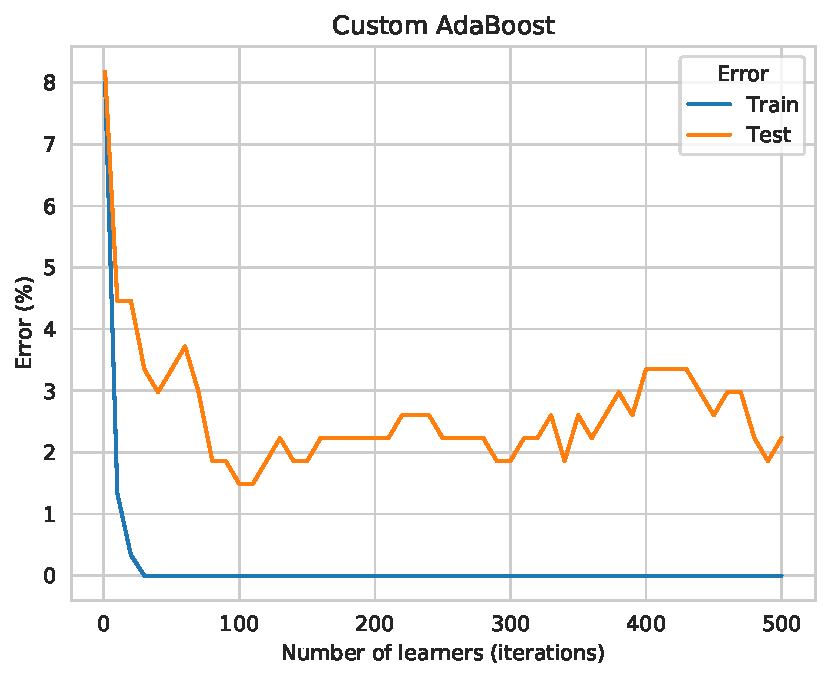
\includegraphics[width=1.0\linewidth]{nlearners_adaboost_custom.pdf}
		\caption{Training and test error of the custom implementation of the AdaBoost algorithm using different number of learners}
		\label{fig:nlearners_adaboost_custom}
	\end{center}
\end{figure}

Despite the relatively good performance showed by the custom AdaBoost implementation, the training time of the algorithm is high (Figure \ref{fig:time_custom}) (conditions tested using Python 3.7.7 in a Ubuntu OS Laptop with 16 gb of RAM and Intel(R) Core(TM) i5-7300HQ CPU @ 2.50GHz processor), showing a training time of 6.1 second using just 10 weak learners and 284.49 seconds (approximately 4.7 minutes), making this model inviable to work in production in certain cases such a large databases.

\begin{figure}[h]
	\begin{center}
		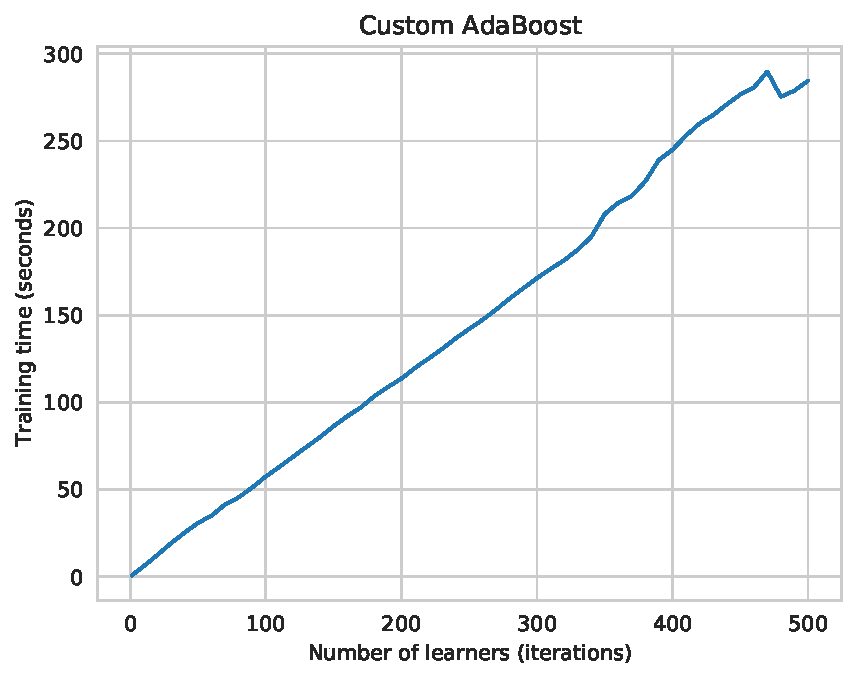
\includegraphics[width=1.0\linewidth]{train_time_custom.pdf}
		\caption{Training time of the custom implementation of the AdaBoost algorithm using different number of learners}
		\label{fig:time_custom}
	\end{center}
\end{figure}

The high prediction accuracy and the large train time can be explained by the greedy nature of the decision stump implemented in this paper, that test each value contained in the dataset for possible thresholds, while at the same time testing for 2 polarity values. In the case of the training data (300 samples and 30 features), this can mean $300*30*2 = 18000$ values that are tested in each decision stump, making the learner produce accurate results but in a long training time.

\section{Third Party AdaBoost Implementation: \textit{Scikit-learn}}

In order to compare the custom AdaBoost implemented in this paper with a commonly used off the shelf implementation, a third party library was used to solve the classification problem. In this case, the \textit{Scikit-learn} library was chosen due to its wide popularity in the machine learning community.

\textit{Scikit-learn} is a Python library that integrates various tools for statistics and machine learning applications, that include classification, regression, metrics and feature selection, among many others. This library is distributed under a BSD licence and includes compiled code, that makes it very efficient. The library is built using other popular numerical Python libraries, such as \textit{Numpy} and \textit{Scipy} \cite{Pedregosa2011}.

According to the library documentation, the AdaBoost classification algorithm that is implemented in this package use the Multi-class Adaboost algorithm variation introduced by Zhu \textit{et al} \cite{Zhu2009}. In this algorithm, the authors modified the originally proposed two class AdaBoost \cite{Freund1999} to include multiple class problems without separating the problem into several two class problems.

In this algorithm, called SAMME, the procedure allows for the classification problem to deal with a set of $K$ distinct classes in the target variable. As follows \cite{Zhu2009}:

Firstly, the weights are initialized as $W_1 = 1/n$. 

Then for each iteration of the algorithm $m = 1,2,3...M$:

- Train a weak learner $G_m(x)$ using the weights $W_m$

- Calculate the error using:

\begin{equation}
	err_m = \frac{\sum_{i=1}^{N} W_i I(y_i \neq G_m(x_i))}{\sum_{i=1}^{N} W_i} 
\end{equation}

- Calculate the $\alpha$ value as

\begin{equation}
	\alpha_m = ln(\frac{1-err_m}{err_m}) + ln(K-1)
\end{equation}

-Update the weights of the samples using the following equation, that results in the weights adding  a total of 1:

\begin{equation}
	W_{m+1} (i) = \frac{W_m exp(-\alpha_m y_i g_m(x_i))}{\sum_{i=1}^{N} W_i}
\end{equation}

Then, to generate the prediction, the maximum number on each of the $k$ categories is used

\begin{equation}
	G(X) = argmax(\sum_{m=1}^{M} \alpha_m g_m(x) I(g_m(x) = k))
\end{equation}

In this case, as the SAMME algorithm \cite{Zhu2009} is being used for a two class classification problem ($K = 2$), the term $ln(K+1)$ in equation 9 becomes zero, making the calculation of $/alpha$ the same as in the custom AdaBoost implemented in this paper.

In order to make a comparison y similar terms, the base learner that was applied is the decision tree implemented in the \textit{Scikit-learn} package, using a depth of 1, making the learner a decision stump in practice. 


\subsection{Experimental results}


The \textit{Scikit-learn} implementation of the AdaBoost algorithm, similarly to the custom implementation, reach a minimum test error of 1.86\% using 110 iterations, and reaching 0\% train error with 30 iterations (Figure \ref{fig:nlearners_adaboost_sklearn}), just as in the custom implementation. After reaching the minimum text error, the \textit{Scikit-learn} implementation do not show a significant overfitting effect, not presenting errors greater than 3\% after iteration 140. 

\begin{figure}[h]
	\begin{center}
		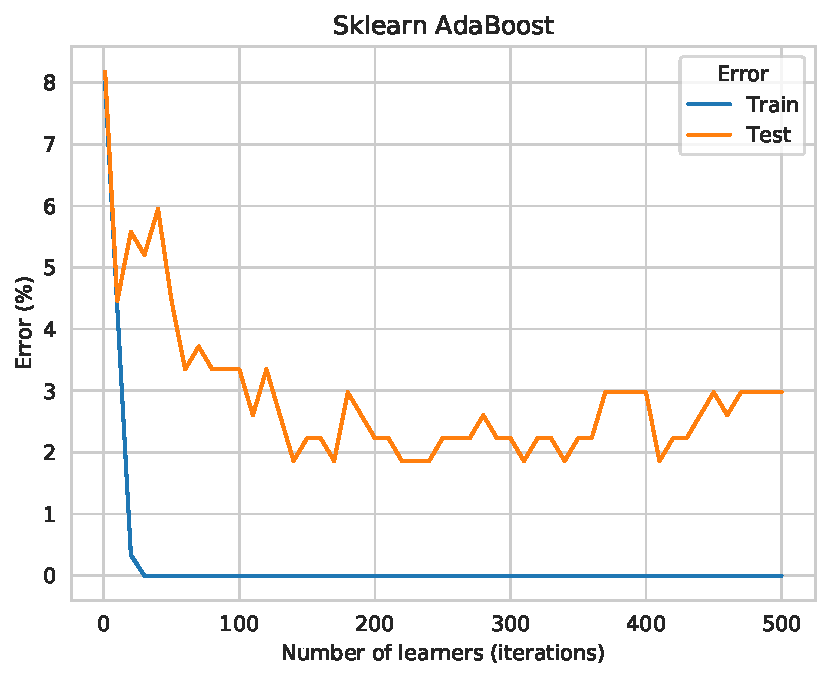
\includegraphics[width=1.0\linewidth]{nlearners_adaboost_sklearn.pdf}
		\caption{Training and testing error of the \textit{Scikit-learn} implementation of the AdaBoost algorithm using different number of learners}
		\label{fig:nlearners_adaboost_sklearn}
	\end{center}
\end{figure}

The big advantage of the \textit{Scikit-learn} implementation over the custom implementation is the time it takes to train the algorithm. In this case, the algorithm took 0.02 seconds to train 10 learners, and 1.41 seconds with 500 weak learners. This much better performance can be attributed to the highly optimized characteristic of the \textit{Scikit-learn} programming, that uses Cython (a compiled Python version based on C/C++) for some operations and that han been under developed several years

\begin{figure}[h]
	\begin{center}
		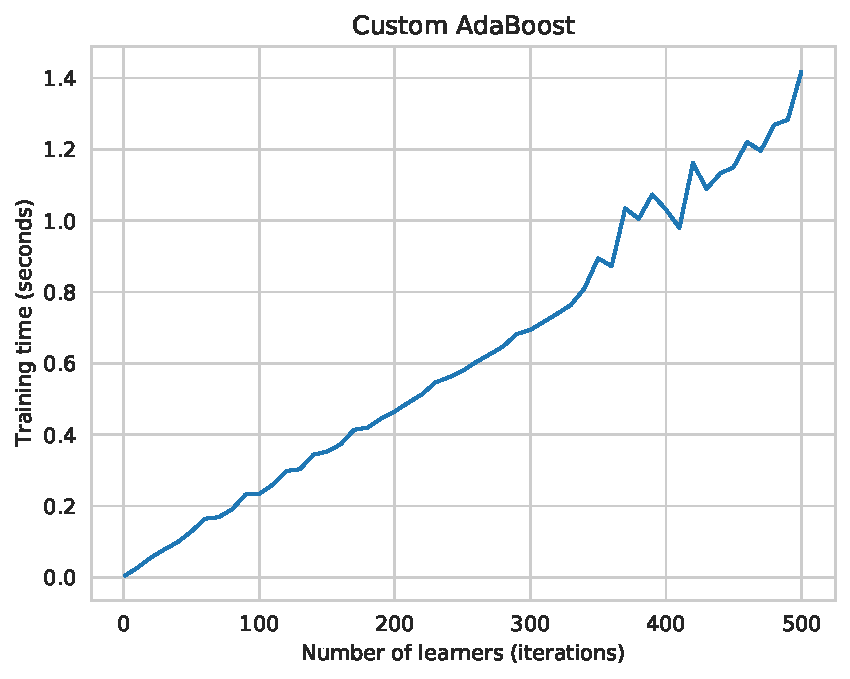
\includegraphics[width=1.0\linewidth]{train_time_sklearn.pdf}
		\caption{Training time of the \textit{Scikit-learn} implementation of the AdaBoost algorithm using different number of learners}
		\label{fig:time_sklearn}
	\end{center}
\end{figure}

\section{Comparison with Support Vector Machine}

The AdaBoost implementations were compared with the Support Vector Machine classification algorithm. This supervised classification algorithm was developed by Vapnik \cite{Vapnik1995}, and consist in an hyperplane that separates a high dimensional space defined by the input variables into discrete classes. This hyperplane is defined to have the largest possible distances to the closest point of either class , thus, maximizing the margin between two classes. The Support Vector Machine has been extensively used in classification problems, as it can include a custom kernel, that can handle non linearly separable cases \cite{Hastie2009}.

In this study, the AdaBoost methods were compared with the \textit{Scikit-learn} package implementation of the Support Vector Machine classifier, using different kernel functions to better adjust the data. The algorithm was tested using different cost values from 0.1 to 10, and testing a linear, polynomial of degree equal to three and radial kernels.

\subsection{Experimental results}

The results of the \textit{Scikit-learn} Support Vector Machine implementation (Figure \ref{fig:svm}) show that in this case the best overall results are presented by using a linear kernel. In this case, the smaller test error (4.09\%) is accomplished using a cost equal to 2.0 on the linear kernel, while the the radial and polynomial kernel reach worse results, in general above 5\% of error.

\begin{figure}[h]
	\begin{center}
		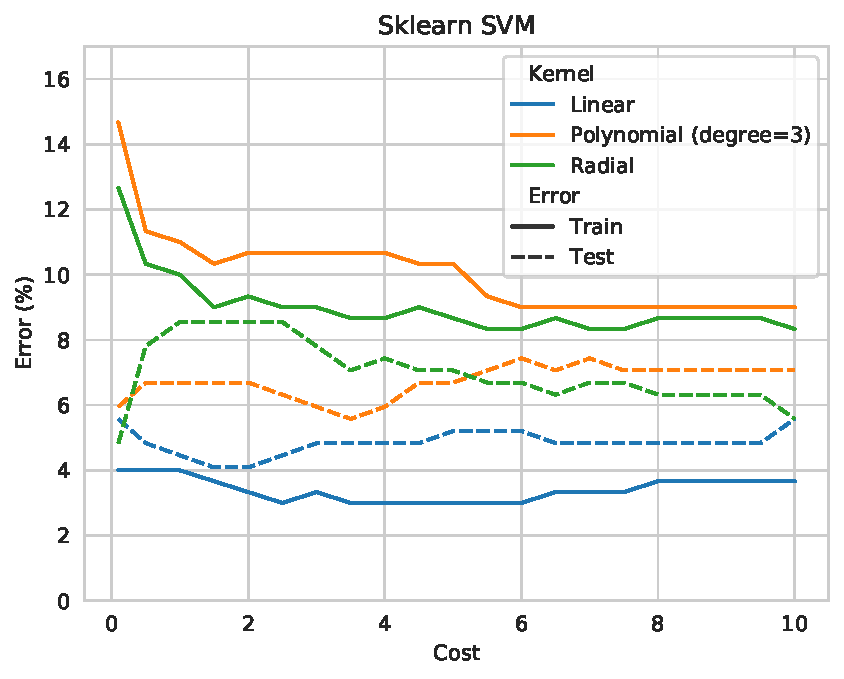
\includegraphics[width=1.0\linewidth]{cost_kernel_svm.pdf}
	\end{center}
	\caption{Training and testing error using different cost and kernel values}
	\label{fig:svm}
\end{figure}

If we compare the SVM results with the the best test error results (Table \ref{table:results}), show that the custom implementation reached a slightly smaller test error, that can be attributed to the greedy approach that was used to code the decision stump, that also caused the algorithm perform several times slower than the third party implementation

On the other hand, the SVM algorithm, despite testing several cost values and types of kernels, did not accomplished to accurately predict the breast cancer class, being outperformed by the AdaBoost algorithms. Although performing faster than the custon AdaBoost implementation

\begin{table}[h]
	\begin{center}
		\begin{tabular}{|p{4cm}|p{1.5cm}|p{1.5cm}|}
			\hline
			Algorithm & Best test error (\%) & Training time (sec.) \\
			\hline\hline
			Custom AdaBoost (110 learners) & 1.49\% & 60.11\\
			\textit{Scikit-learn} AdaBoost (140 learners)& 1.86\% & 0.38\\
			\textit{Scikit-learn} SVM (linear kernel and cost = 1.5) & 4.09\% & 1.34\\
			\hline
		\end{tabular}
	\end{center}
	\caption{Best test results for the implemented algorithm}
	\label{table:results}
\end{table}

To find an explanation to this results a Principal Components analysis was performed as a visualization tool, using the complete dataset to check the separability of the classes. In Figure \ref{fig:pca} it is possible to see that the classes do not present a clear separable boundary, making algorithms such as SVM, that depend of a specific function type, less likely to perform well, on the other side, the AdaBoost algorithm is capable of creating a "flexible" boundary between classes, hence performing better in this case.

\begin{figure}[h]
	\begin{center}
		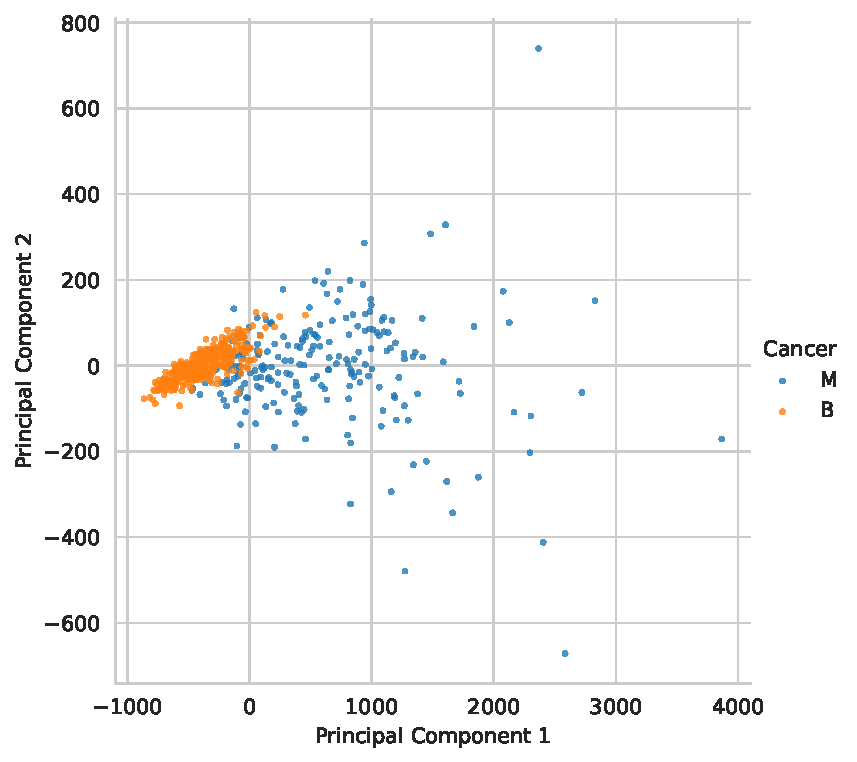
\includegraphics[width=1.0\linewidth]{pca.pdf}
	\end{center}
	\caption{Principal component analysis of the dataset}
	\label{fig:pca}
\end{figure}

\section{Code}

The code to reproduce this project was attached to this report. The primal and dual implementations of the models were programmed in Python 3.7 using only commonly used libraries such as numpy for numerical computation, pandas for the reading of databases and copy and os for general utilities.

As the  testing of different number of learners in the case of the AdaBoost algorithm, or the testing of several C values and kernels in the case of SVM can take several hours (depending of the computing power of the equipment), the codes of the different implementations contain the saving of the results into a .csv file, that contains the results of the different parameter testing

The instructions to run the attached codes can be found in the accompanying README.txt file.


{\small
\bibliographystyle{ieeetr}
\bibliography{library}
}


\end{document}



